\documentclass[11pt]{article}

\usepackage[margin=1in]{geometry}
\usepackage{booktabs}
\usepackage{amsmath}
\usepackage{amssymb}
\usepackage{amsthm}
\usepackage{verbatim}
\usepackage{graphicx}
\usepackage{xcolor}
\usepackage[round,authoryear]{natbib}
\usepackage[colorlinks=true,allcolors=blue]{hyperref}
\usepackage{caption}
\captionsetup{font=small,labelfont=bf}

\newcommand{\code}[1]{\texttt{#1}}
\newtheorem{proposition}{Proposition}

\title{\textbf{Measuring Leakage, Not Learning:\\
Structural Label Leakage in Cloud-Resource\\ Attribution Benchmarks}}

\author{Parth Auti\\
\small Independent \quad\textbar\quad \href{https://github.com/pauti04/CostDNA}{\code{github.com/pauti04/CostDNA}}}

\date{2026 \quad\textbar\quad Preprint}

\begin{document}
\maketitle

\begin{abstract}
\noindent
Cloud-resource attribution, the task of recovering which team or service owns
each resource in a mostly-untagged account, is often cast as graph node
classification, and published accuracies on cluster traces fall in the 85 to
97 percent range. We trace these numbers to structural label leakage. The
identifier columns commonly used to build graph edges (deployment, user, and
collection IDs) are near-deterministic functions of the attribution target, so
label propagation over such an edge reduces prediction to a lookup. We make the
effect precise with a determinism measure and show, in theory and in a
controlled experiment, that label-propagation accuracy is lower-bounded by and
empirically equal to the determinism of the edge. Auditing three cluster traces
from two providers gives the same result each time. On Microsoft's Azure trace,
\code{deployment\_id} identifies the subscription for all 33{,}205 deployments
and label propagation reaches 97 percent; removing the edge leaves GraphSAGE at
6.9 percent on 100-class attribution. On Microsoft's Philly trace,
\code{user\_id} is 94.6 percent deterministic and GraphSAGE drops from 34 to 11
percent. On Google's Borg trace, \code{collection\_id} determines scheduling
priority and label propagation drops from 83 to 28 percent. The audit also
flags our own synthetic benchmark, which we discuss rather than quietly exclude.
We release the post-audit baselines, the harness, and a small package that runs
the check in one line. On this evidence, cloud-attribution benchmarks measure
leakage more than they measure learning.
\end{abstract}

\section{Introduction}

Public cloud accounts accumulate resources faster than they accumulate
governance. On a typical account, 40 to 60 percent of spend is untagged: the
line item and the dollars are real, but nothing records which team owns the
resource. Downstream cost tools read tags, so untagged spend collapses into one
opaque bucket. Cloud-resource attribution is the task of recovering the missing
owner from behavioral signals such as API-call patterns, access patterns, cost
time-series shape, and network or scheduling structure.

Resources and their interactions form a graph, so attribution is naturally
posed as node classification, and graph neural networks such as GraphSAGE
\citep{hamilton2017graphsage} are an obvious tool. Published accuracies on
cloud traces are high, often between 85 and 97 percent. On a problem with tens
to hundreds of classes, a number that high is a reason for suspicion before it
is a reason for confidence.

We argue, and show on three traces, that the high numbers are mostly an
artifact of structural label leakage. Cloud datasets carry identifier metadata
such as deployment, request, user, and collection IDs, and it is convenient to
wire these in as graph edges. Such a column is not an independent behavioral
signal. It is a near-deterministic function of the target, for a structural
reason: organizations provision resources in units, and each unit sits under a
single owner. A deployment belongs to one subscription; a user submits to one
cluster; a service runs at one priority. When the column becomes a graph edge,
label propagation walks the label along an edge that already encodes it, and no
learning is required.

\paragraph{Contributions.}
\begin{enumerate}
  \item A determinism measure for candidate graph edges, and a proof that
  label-propagation accuracy is lower-bounded by edge determinism. A controlled
  experiment shows accuracy matches determinism almost exactly
  (Section~\ref{sec:method}, Figure~\ref{fig:sweep}).
  \item An audit of three cluster traces from two providers, with honest
  post-audit baselines. Removing a single edge collapses the leading method
  from 97 to 6.9 percent on Azure, 34 to 11 on Philly, and 83 to 28 on Borg
  (Section~\ref{sec:results}).
  \item The same audit applied to our own synthetic benchmark, which it also
  flags, reported openly (Section~\ref{sec:reflexive}).
  \item A reproducible harness, per-dataset scripts, and a \code{pip}
  package that runs the check (Section~\ref{sec:repro}).
\end{enumerate}

The thesis is meant to be falsifiable: across published cloud-attribution
benchmarks, the dominant predictive signal is structural metadata that
determines the target, and behavioral attribution is much weaker than the
literature suggests. Section~\ref{sec:discussion} states the test that would
overturn it. We have not found a case that does.

\section{Background and Related Work}

Leakage, where information about the target reaches the model in a form
unavailable at prediction time or trivially encoding the label, is a long-known
failure mode in applied machine learning \citep{kaufman2012leakage}. Our
subject is a specific form of it: a leak that enters through graph-edge
construction rather than a feature column, in a setting where its structural
origin makes it systematic rather than accidental. Relatedly, models routinely
learn predictive shortcuts instead of the intended signal
\citep{geirhos2020shortcut}; structural leakage is a shortcut with an unusually
clean signature, since the offending edge is close to a lookup table and the
inflated accuracy vanishes the moment the edge is dropped.

We evaluate GraphSAGE \citep{hamilton2017graphsage} against label propagation
\citep{zhu2002labelprop}, a \code{node2vec} embedding \citep{grover2016node2vec}
with logistic regression, and feature-only baselines. Label propagation is the
sharpest diagnostic. It has no learned parameters and reads no features; it only
spreads observed labels across edges, so a leaking edge takes it directly to a
near-perfect score. A GNN inherits a weaker version of the same effect, because
message passing over a within-class edge draws same-class nodes together in
embedding space.

The traces we use were released for systems research on workload prediction and
scheduling: Microsoft's Azure Public Dataset from Resource Central
\citep{cortez2017resourcecentral}, the Philly GPU-cluster trace
\citep{jeon2019philly}, and Google's Borg cluster-usage trace
\citep{tirmazi2020borg}. We repurpose them for attribution, and the leakage we
describe is a property of that repurposing, not a defect in the datasets. Where
we report confidence it is calibrated by temperature scaling
\citep{guo2017calibration}.

\section{The Determinism Audit}
\label{sec:method}

Consider a table with a target column $t$ and a set of candidate columns
$\{c\}$ that could serve as graph edges. Group the rows by the value of $c$ and,
within each group, count the distinct values of $t$. The determinism of $c$
with respect to $t$ is the fraction of $c$-groups that resolve to a single
target value:
\[
  D(c, t) \;=\;
  \frac{\bigl|\{\, v \in \mathrm{vals}(c) \;:\; |\{\, t(r) : c(r) = v \,\}| = 1 \,\}\bigr|}
       {|\mathrm{vals}(c)|}.
\]
When $D(c,t)=1$, every value of $c$ maps to one target value and $c$ is a
perfect lookup of $t$. The audit is two lines of \code{pandas} per candidate:
\begin{quote}
\begin{verbatim}
for c in candidate_edge_cols:
    determinism = (df.groupby(c)[target].nunique() == 1).mean()
    if determinism >= threshold:      # flag c as leaking
        print(c, determinism)
\end{verbatim}
\end{quote}
Our default threshold is $0.85$. Two cases need care. A column with roughly as
many distinct values as rows, such as a primary key, is trivially deterministic;
we mark high-cardinality columns separately, since their score reflects
cardinality rather than a structural leak, though both should be kept out of the
graph. And the audit sees only the columns it is given, so a clean report is
evidence about those columns, not a guarantee about the dataset.

\subsection{Why determinism inflates accuracy}

For label propagation, determinism does more than correlate with accuracy: it
lower-bounds it.

\begin{proposition}
\label{prop:bound}
Let $G$ be the graph whose connected components are the edge-groups of a
candidate column $c$, with minimum group size $k$, and let each node be labeled
in training independently with probability $\rho$. Under majority-vote label
propagation, the expected test accuracy satisfies
\[
  \mathbb{E}[\mathrm{acc}] \;\ge\; D(c,t)\,\bigl(1-(1-\rho)^{k-1}\bigr).
\]
For well-covered graphs this gives $\mathrm{acc}\approx D(c,t)$, so a perfectly
deterministic edge yields near-perfect accuracy without any learning.
\end{proposition}

\begin{proof}[Proof sketch]
Take a test node $u$ in a pure group, one whose members all share $u$'s class.
If $u$ has at least one labeled neighbor, majority vote returns that class and
$u$ is correct. The probability $u$ has a labeled neighbor is
$1-(1-\rho)^{k-1}$. Pure groups are a $D(c,t)$ fraction of all groups by
definition, and mixed groups contribute a nonnegative remainder that we drop.
\end{proof}

\begin{figure}[t]
\centering
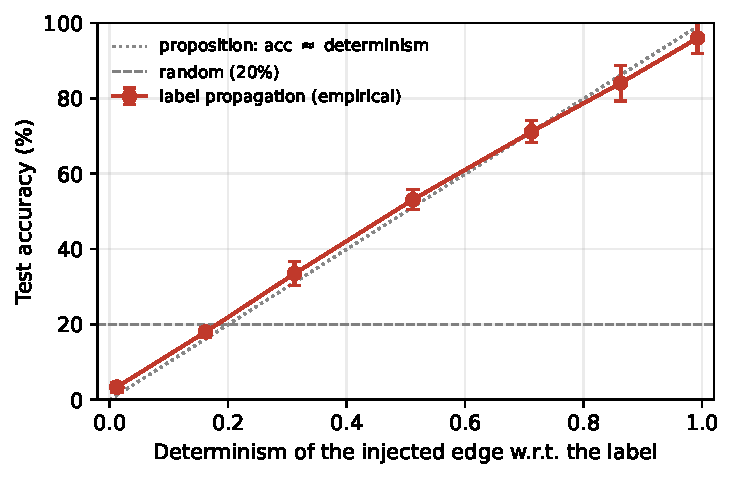
\includegraphics[width=0.6\textwidth]{fig-sweep.pdf}
\caption{Label-propagation accuracy as a function of edge determinism. We inject
a single edge at controlled determinism into a 5-class task (400 nodes,
$\rho=0.7$, group size 4), with node features set to pure noise so the edge is
the only signal, and measure test accuracy over 5 seeds. The empirical curve
tracks the determinism value predicted by Proposition~\ref{prop:bound}: at
$D=0.99$ the bound gives $96.3\%$ and the measurement is $96.0\%$. Below
$D\approx0.2$, a mostly-mixed edge misleads propagation and accuracy falls under
the random floor.}
\label{fig:sweep}
\end{figure}

Figure~\ref{fig:sweep} confirms the bound. With the label as the only usable
signal, label-propagation accuracy rises with edge determinism from below random
to 96 percent, and stays close to the identity line throughout. This is the
mechanism behind the inflated benchmark numbers: on a leaking graph, accuracy is
a readout of edge determinism, and at determinism one there is nothing to learn.

\section{Datasets and Setup}

\paragraph{Azure Public Dataset.} 2.6M virtual machines across 100 subscriptions
over 30 days \citep{cortez2017resourcecentral}; the target is the subscription.
The trace carries summary CPU statistics per VM (max, average, p95) rather than
the full hourly series, so per-resource features are thin.

\paragraph{Philly GPU-cluster trace.} 117K deep-learning jobs across virtual
clusters \citep{jeon2019philly}; the target is the virtual cluster. We take the
top 15 clusters, at most 200 jobs each, for 2{,}317 jobs.

\paragraph{Google Borg trace.} Instance events from Google's cluster-usage
release \citep{tirmazi2020borg}. Borg is anonymized and has no team field, so we
predict an instance's scheduling priority (5 tiers) from its resource request,
balanced to at most 400 instances per tier. This is a proxy for ownership,
chosen to exercise the same structural pattern on a third trace.

\paragraph{Synthetic environment.} A controlled generator with a configurable
class count and injected hard cases, used for the mechanism experiment of
Section~\ref{sec:method} and for the ablation in Section~\ref{sec:reflexive}.

\paragraph{Models.} GraphSAGE uses four \code{SAGEConv} layers with mean
aggregation, hidden dimension 16, and an input projection with residual
connections, trained with AdamW (weight decay $5\times10^{-4}$) under
cross-entropy for up to 200 epochs with early stopping. Baselines are logistic
regression with balanced class weights, $k$-NN with $k=5$, label propagation,
and \code{node2vec} embeddings from biased random walks
\citep{grover2016node2vec} with logistic regression. Accuracy is a stratified
70/30 split averaged over the seeds listed in each script; chance is $1/N$ for
$N$ classes.

\section{Results}
\label{sec:results}

\subsection{Azure}

The audit flags \code{deployment\_id} at determinism $1.000$: across all
33{,}205 deployments, each belongs to exactly one subscription. As a graph edge
it takes label propagation to 97 percent on 100-class attribution, which is a
join rather than a prediction. With the leaking edges removed
(Table~\ref{tab:azure}), GraphSAGE reaches $6.9\pm0.5$ at 100 classes, about
seven times the 1 percent floor and ahead of every baseline, but an order of
magnitude below the leaked figure.

\begin{table}[h]
\centering
\caption{Azure post-audit test accuracy (\%), leaking edges removed. Chance
$=1/N$.}
\label{tab:azure}
\begin{tabular}{rrrrrrr}
\toprule
$N$ subs & Chance & Majority & LogReg & $k$-NN & LabelProp & \textbf{GraphSAGE} \\
\midrule
5   & 20.0 & 17.2 & 31.3 & 28.6 & 20.0 & \textbf{34.6} \\
10  & 10.0 &  8.4 & 18.3 & 17.3 & 10.0 & \textbf{22.5} \\
25  &  4.0 &  3.3 &  9.2 & 10.0 &  4.0 & \textbf{10.6} \\
50  &  2.0 &  1.6 &  5.8 &  6.2 &  2.0 & \textbf{9.2}  \\
100 &  1.0 &  0.7 &  3.4 &  3.8 &  1.0 & \textbf{6.9}  \\
\bottomrule
\end{tabular}
\end{table}

\subsection{Philly}

On a trace with a different domain, target, and team, the audit flags
\code{user\_id} at determinism $0.946$: about 95 percent of users submit to a
single cluster. The honest machine edge scores $0.144$. Removing the user edge
drops GraphSAGE from 34 to 11 percent at 15 clusters (Table~\ref{tab:philly}).
One detail is worth stating against our own interest: on the de-leaked graph
GraphSAGE does not win. Label propagation ($17.6\pm1.5$) and \code{node2vec}
($13.4\pm0.6$) both beat it ($11.3\pm1.0$). Once the shortcut is gone, every
method sits in the low teens, which is the point.

\begin{table}[h]
\centering
\caption{Philly: GraphSAGE with the leaking \code{user\_id} edge and with it
removed. Dropping one edge roughly thirds the accuracy.}
\label{tab:philly}
\begin{tabular}{rrrrr}
\toprule
$N$ clusters & Chance & Leaky & \textbf{De-leaked} & Ratio to chance \\
\midrule
3  & 33.3 & 91.2 & \textbf{54.4} & $1.6\times$ \\
5  & 20.0 & 62.2 & \textbf{35.4} & $1.8\times$ \\
10 & 10.0 & 42.9 & \textbf{18.4} & $1.8\times$ \\
15 &  6.7 & 34.2 & \textbf{11.3} & $1.7\times$ \\
\bottomrule
\end{tabular}
\end{table}

\subsection{Google Borg}

The audit flags \code{collection\_id} at determinism $1.000$ of priority, since
every instance in a service runs at one tier, and \code{machine\_id} at
$0.923$. Table~\ref{tab:google} shows the collapse when the \code{collection\_id}
edge is removed: the propagation methods, label propagation at 83 percent and
\code{node2vec} at 78, fall to the 28 percent feature floor. Priority is close
to unpredictable from the resource request alone, and nearly all of the apparent
signal was the edge.

\begin{table}[h]
\centering
\caption{Google Borg, predicting scheduling priority (5 tiers, chance $=20\%$),
with the leaking \code{collection\_id} edge and with it removed.}
\label{tab:google}
\begin{tabular}{lrr}
\toprule
Model & Leaky & \textbf{De-leaked} \\
\midrule
Majority             & 27.6 & 27.6 \\
LogReg               & 27.8 & 27.8 \\
$k$-NN ($k{=}5$)     & 27.8 & 27.8 \\
LabelProp            & \textbf{83.4} & \textbf{27.8} \\
\code{node2vec}$+$LR & 77.8 & 27.8 \\
GraphSAGE            & 36.2 & 23.3 \\
\bottomrule
\end{tabular}
\end{table}

\subsection{The pattern across traces}

Table~\ref{tab:cross} collects the three cases. The traces come from two
companies and use three different targets, yet each has an identifier column
that determines the target and carries most of the reported accuracy.

\begin{table}[h]
\centering
\caption{The same signature on three traces from two providers. ``Inflated'' is
the leading graph method with the leaking edge present; ``honest'' is the best
method with it removed.}
\label{tab:cross}
\begin{tabular}{llrlrl}
\toprule
Trace & Provider & Classes & Leaking edge & Determinism & Inflated $\rightarrow$ honest \\
\midrule
Azure  & Microsoft & 100 & \code{deployment\_id} & 1.000 & LabelProp 97\% $\rightarrow$ 6.9\% \\
Philly & Microsoft & 15  & \code{user\_id}       & 0.946 & GraphSAGE 34\% $\rightarrow$ 11\% \\
Borg   & Google    & 5   & \code{collection\_id} & 1.000 & LabelProp 83\% $\rightarrow$ 28\% \\
\bottomrule
\end{tabular}
\end{table}

\subsection{The audit on our own benchmark}
\label{sec:reflexive}

We ran the determinism check on our own synthetic benchmark. It flags
\code{vpc\_cidr} and \code{iam\_role} at $1.000$, the same score we call a leak
on Azure. This is deliberate: the generator models real structure, with each
team on its own VPC and role names that follow team conventions, and both
columns feed the graph. We report it rather than exclude it. The audit cannot,
on its own, separate a benchmark artifact from modeled structure; by its own
numeric standard both trip the threshold. Two facts keep the synthetic results
usable. An edge-dropout ablation gives 89.4 percent with the graph removed
entirely, so the headline does not rest on the deterministic edges, and we treat
synthetic numbers as ablations rather than claims. The tool now runs this audit
on its inputs before training and warns when a column determines the label.

\subsection{A non-leaking validation}

To check that behavioral attribution works when features are rich, we
provisioned a real AWS account with full CloudTrail through infrastructure as
code, hand-labeled 15 resources across three teams, and ran the pipeline end to
end. It was correct on 13 of 15 (87 percent; 95 percent Wilson interval
$[62,96]$), and on 13 of 14 high-confidence predictions (93 percent, $[69,99]$);
the two errors both fell below the confidence threshold and were routed to human
review by design. With 15 labels this is engineering evidence, not a
methodological result, but it indicates that the collapse on public traces comes
from thin features and structural leakage rather than from the approach.

\section{Discussion}
\label{sec:discussion}

\paragraph{Why the pattern recurs.} Structural leakage is not a vendor bug but a
consequence of how cloud resources are created. Teams provision resources inside
deployments, submit jobs as users, and run services as collections, and each
unit is scoped to one subscription, cluster, or priority. The identifier
metadata therefore encodes the org chart, which is the attribution target.
Finding the same signature on three unrelated traces from two companies is what
a structural cause predicts.

\paragraph{The falsifiable claim.} We claim that published cloud-attribution
results built on deployment, request, user, or collection identifiers report
accuracies inflated by structural leakage, and that honest behavioral accuracy
on many-class problems is in the single digits to mid teens. A single
counterexample settles it: a cloud-attribution result that runs the determinism
audit, excludes the leaking edges, and still reports high accuracy. We have
looked and not found one.

\paragraph{A reporting standard.} We suggest that cloud-attribution results
report, next to their accuracy, the determinism of every column used as an edge.
It costs one line per column, and by Proposition~\ref{prop:bound} it turns an
unfalsifiable headline into a checkable one.

\section{Threats to Validity}

The determinism measure treats a column as a leak when its values map to single
targets, which also flags a legitimate feature that happens to be single-use,
such as a unique key. The high-cardinality marker mitigates this, but the audit
is a screen and not a verdict: a flagged column deserves inspection, not
automatic deletion. The mechanism experiment uses noise features to isolate the
edge, so its clean linear relation bounds the leakage contribution rather than
total accuracy, and holds specifically for label propagation. Finally, three
traces are not the field. Our statement about prior work is an inference from
the mechanism and three data points, not a re-audit of specific systems, and the
Borg priority target is a proxy for ownership rather than ownership itself.

\section{Limitations}
\label{sec:limitations}

Public traces carry thin, summary-level features, so the modest margin of
GraphSAGE over feature-only baselines partly reflects feature poverty; we cannot
measure the rich-feature regime on public data, because we know of no public
trace that has both rich per-resource behavior and no structural leak, which is
itself a gap worth filling. The real-AWS validation rests on 15 labels and a
wide interval. We do not re-run prior systems. The synthetic environment is
synthetic and, as reported, trips its own audit by construction.

\section{Reproducibility}
\label{sec:repro}

Every result reproduces from the open-source repository. The audit ships as a
tested package:
\begin{quote}
\begin{verbatim}
pip install leakaudit
leakaudit data.csv --target subscription_id --fail-on-leak   # CI gate
\end{verbatim}
\end{quote}
Per-dataset scripts (\code{bench-azure.py}, \code{bench-philly.py},
\code{bench-google.py}, \code{bench-determinism-sweep.py}) regenerate each table
and the figure, emitting the leaky and de-leaked configurations together, and
the reflexive synthetic audit is fixed by a regression test. The protocol is a
stratified 70/30 split, up to 200 epochs with early stopping, and multiple
fixed seeds with reported standard deviations. Code, data pointers, and the
harness are at
\href{https://github.com/pauti04/CostDNA}{\code{github.com/pauti04/CostDNA}}.

\section{Conclusion}

Cloud-resource attribution looks close to solved on public benchmarks and is
not. The high numbers come from identifier metadata that determines the target
and, used as a graph edge, replaces learning with a lookup. We characterized the
effect with a determinism measure and a lower bound, confirmed it in a
controlled experiment, and found the same signature on three traces from two
providers and on our own benchmark. Behavioral attribution is real but modest:
about seven times chance at 100 classes on Azure, under two times chance at 15
clusters on Philly, and at the feature floor on Borg. We release the audit, the
honest baselines, and the harness, and we ask for one number alongside future
accuracies: the determinism of every edge against the target.

{\small
\bibliographystyle{plainnat}
\begin{thebibliography}{99}

\bibitem[Cortez et al.(2017)]{cortez2017resourcecentral}
E.~Cortez, A.~Bonde, A.~Muzio, M.~Russinovich, M.~Fontoura, and R.~Bianchini.
\newblock Resource Central: Understanding and predicting workloads for improved
resource management in large cloud platforms.
\newblock In \emph{SOSP}, 2017.

\bibitem[Geirhos et al.(2020)]{geirhos2020shortcut}
R.~Geirhos, J.-H. Jacobsen, C.~Michaelis, R.~Zemel, W.~Brendel, M.~Bethge, and
F.~A. Wichmann.
\newblock Shortcut learning in deep neural networks.
\newblock \emph{Nature Machine Intelligence}, 2(11):665--673, 2020.

\bibitem[Grover and Leskovec(2016)]{grover2016node2vec}
A.~Grover and J.~Leskovec.
\newblock node2vec: Scalable feature learning for networks.
\newblock In \emph{KDD}, 2016.

\bibitem[Guo et al.(2017)]{guo2017calibration}
C.~Guo, G.~Pleiss, Y.~Sun, and K.~Q. Weinberger.
\newblock On calibration of modern neural networks.
\newblock In \emph{ICML}, 2017.

\bibitem[Hamilton et al.(2017)]{hamilton2017graphsage}
W.~L. Hamilton, R.~Ying, and J.~Leskovec.
\newblock Inductive representation learning on large graphs.
\newblock In \emph{NeurIPS}, 2017.

\bibitem[Jeon et al.(2019)]{jeon2019philly}
M.~Jeon, S.~Venkataraman, A.~Phanishayee, J.~Qian, W.~Xiao, and F.~Yang.
\newblock Analysis of large-scale multi-tenant GPU clusters for DNN training
workloads.
\newblock In \emph{USENIX ATC}, 2019.

\bibitem[Kaufman et al.(2012)]{kaufman2012leakage}
S.~Kaufman, S.~Rosset, C.~Perlich, and O.~Stitelman.
\newblock Leakage in data mining: Formulation, detection, and avoidance.
\newblock \emph{ACM TKDD}, 6(4):1--21, 2012.

\bibitem[Tirmazi et al.(2020)]{tirmazi2020borg}
M.~Tirmazi, A.~Barker, N.~Deng, M.~E. Haque, Z.~G. Qin, S.~Hand,
M.~Harchol-Balter, and J.~Wilkes.
\newblock Borg: the next generation.
\newblock In \emph{EuroSys}, 2020.

\bibitem[Zhu and Ghahramani(2002)]{zhu2002labelprop}
X.~Zhu and Z.~Ghahramani.
\newblock Learning from labeled and unlabeled data with label propagation.
\newblock Technical Report CMU-CALD-02-107, Carnegie Mellon University, 2002.

\end{thebibliography}
}

\end{document}
